\section{Design considerations}
\label{sec:design_considerations}

\subsection{Background and context}
\label{sec:background_context}

\textit{Quantum nodes}.
A quantum internet connects quantum nodes on which quantum programs may be 
executed.
%(Figure~\ref{fig:qoala_location}). 
In their most general form, such nodes
are \textit{processing nodes} that have a quantum memory to store quantum bits (qubits) on which quantum operations (qubit initialization, quantum gates and measurements) can be performed. Pairs of nodes can establish \textit{entanglement} between them over a quantum network. Entanglement is a special property of two qubits (an \emph{entangled pair}), where one qubit is stored in the memory of each node. Nodes can also exchange classical messages (e.g. via dedicated classical links or the internet), where no guarantees are assumed on their message delivery times. 

\textit{Programs}.
A program is a series of instructions to be executed by a node.
Instructions can be categorized into four types: local classical processing, classical message-passing, quantum local processing (quantum operations), and remote entanglement generation.
A program can keep classical variables in a classical memory, and quantum variables (qubits) in the node's quantum memory during the execution.
Multiple programs, each running on their own node, together form an \textit{application} (see~\ref{fig:program_illustration}), e.g. QKD (two programs, one per node),
or secret sharing~\cite{hillery1999quantum} (a program each on many nodes).
Programs may involve asynchronous operations (e.g. a server awaiting entanglement with multiple clients).

\textit{Network schedule}.
A quantum network stack has been proposed~\cite{dahlberg2019link} and implemented~\cite{pompili2022experimental} that turns entanglement generation into a robust service independent of the quantum hardware platform.
Important for the design of an architecture for the execution of quantum internet applications is that in this stack, the nodes will establish a network schedule of time slots in which they will trigger entanglement generation (due to need to synchronize entanglement generation at the physical layer~\cite{dahlberg2019link} at high-precision (ns)).
This means that once entanglement has been requested from the network, the nodes can use only the slots in the network schedule to produce entanglement between them, imposing constraints on the ability to schedule applications. What's more, in present day systems~\cite{pompili2021realization, krutyanskiy2023entanglement} limitations in the physical devices prohibit the execution of local operations while engaging in network operations (entanglement generation), creating further dependencies between the local quantum execution and entanglement generation. 
As the specifics of network scheduling~\cite{network-scheduling, skrzypczyk2021architecture} are not within scope of this paper,
we assume the existence of a \textit{network controller} that takes application demand for entanglement and issues a network schedule to the nodes. 
A schedule consists of sequential time slots, each with a start time and duration, when the node will trigger entanglement generation.
Nodes are not forced to attempt entanglement in corresponding time slots, and can instead choose to do local processing instead.

%\begin{figure}[ht]
%    \centering
    %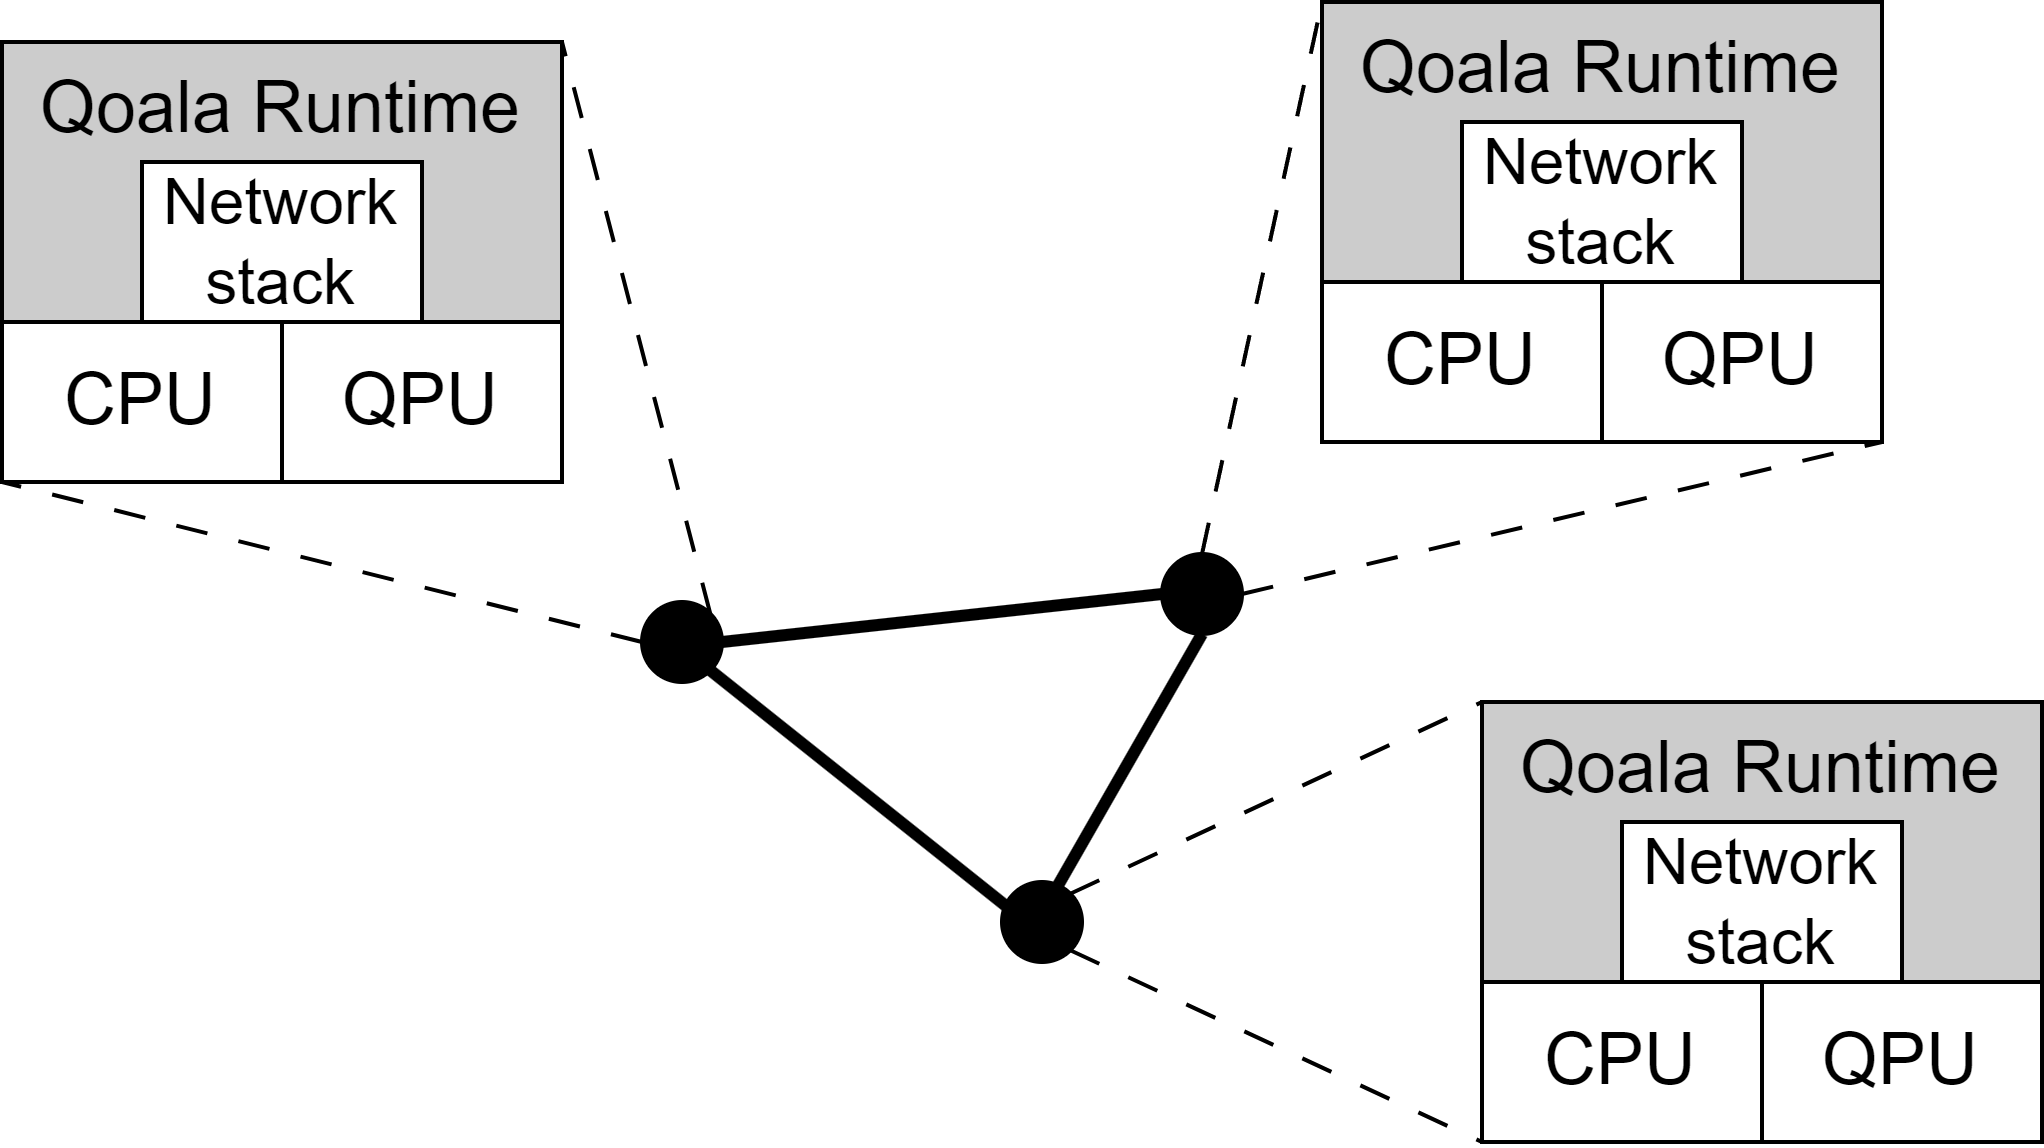
\includegraphics[width=\columnwidth]{figures/qoala_location.png}
    %\caption{
        %Each node in the quantum internet has its own instance of a Qoala runtime environment, which uses its classical (CPU) and quantum processing (QPU) capabilities, as well as the network stack.
    %}
    %\label{fig:qoala_location}
%\end{figure}

\textit{Performance metrics and noise}. Quantum internet applications have classical outcomes that are typically probabilistic in nature:
(1) applications may intentionally do measurements on quantum states that have fundamentally probabilistic outcomes (e.g. quantum cryptography),
(2) in practice, quantum hardware is imperfect (or \textit{noisy}). That is, undesired errors occur
when performing operations (such as gates, measurements, or entanglement generation) or when keeping quantum states in memory for too long.

In many quantum internet applications (e.g. BQC), a single execution of the application can result in failure or success (e.g. a BQC client receives correct measurement results from the server program~\cite{leichtle2021verifying}). Applications are often executed many times, where outcome statistics are computed in order to validate successful execution (e.g. by majority of outcomes).
We consider two metrics:
a \emph{quantum metric} -  the \textit{success probability} of executing a single instance of the application (on average), and a \emph{classical metric} -  the \textit{makespan}, i.e. the average execution time of an application instance.

\subsection{Considerations}
Considerations can be categorized into three main groups: fundamental, technological, and enabling.

\noindent\textit{\textbf{Fundamental Considerations}}
(1) \textit{Hybrid nature of applications}: Quantum internet applications inherently consist of both classical and quantum segments, as well as local and networking operations. The execution environment must account for this hybrid nature, and the program structure should accommodate all types of operations.
(2) \textit{Interactive nature of applications}: Quantum internet applications require classical communication between nodes. This communication may take place in between classical and quantum segments of a single program. 
This implies the need for application-level interfaces between programs on different nodes, and for interfaces between classical and quantum code segments on a single node.
(3) \textit{Multitasking}: Programs may spend a significant amount of time waiting for messages from a remote node (ms), motivating multitasking to make optimal use of the classical and quantum computing resources at each node.  This requires scheduling of time and resources.

\noindent\textit{\textbf{Technological Considerations}}
(1) \textit{Limited qubit lifetime}:
Quantum memory quality degrades over time, presenting a significant challenge for the execution environment,
especially in near-term hardware (ms to s memory lifetimes~\cite{ruf2021quantum, pompili2021realization, krutyanskiy2023telecom}).
As such, there are natural deadlines to application execution after which a desired performance (success probability) can no longer be reached.
We thus desire that a program specification allows indication of memory quality constraints (deadlines), which the runtime environment can act upon (e.g. by appropriate scheduling or restarting).
(2) \textit{Integration of processing and networking}: We assume that near-term nodes only have a single quantum processor, which needs to perform both local quantum gates as well as remote entanglement generation.
That is, while performing local operations the processor is blocked from networking operations and vice versa, as is the case for all current implementations~\cite{pompili2021realization, krutyanskiy2023entanglement} but may be mitigated partially using future proposals~\cite{vardoyan2022quantum}. 
The node must hence allocate time for local computation while at the same time adhering to the network schedule which constrains timing of the entanglement operations.

\noindent\textit{\textbf{Enabling Considerations}}
(1) \textit{Different compilation strategies and programming languages}: The execution environment should support various compilation strategies and accessible programming languages. 
In order to enable compilation, we furthermore want a representation of the program that can be integrated with existing compiler frameworks.
(2) \textit{Different scheduling strategies}: Since we expect that scheduling plays a vital role in optimizing application performance, the execution environment should enable scheduling, and support different scheduling algorithms and policies, 
allowing for their comparison and evaluation.
(3) \textit{Different (control) hardware implementations}: The architecture should make minimal assumptions on the classical control hardware, and be independent on the choice of quantum hardware platform~\cite{carlothesis},
allowing for integration with multiple (future) technologies such as NV centers~\cite{pompili2022experimental} or trapped ions~\cite{drmota2023robust}.

